\subsection{Stopped Proton}

When we indicate the validity of charge response in high dE/dx region, proton is good sample due to its simple event structure.
At the same time, we verificate the recombination factor by proton in this analysis because proton has wide dE/dx range, and this is meaningless if the charge response of MC doesn't agree with that of DATA.
Therefore proton is very impotant in terms of comprehension of charge response.\\
Figure\ref{fig:various_distibution} shows the comparison of the distribution of Hit Charge, Hit Sigma, Stopped Channel and  Cluster Charge between DATA and MC.
Hit Charge shows the distribution of the integral which fit signal wave form  with gaussian.
Hit Sigma shows the distribution of all the dispersion which fit signal wave form with gaussian.
Cluster Charge shows the sum of the Hit integral of the cluster which is selected as good proton event.
All four distribution of MC reproduce DATA well.
Especially, the agreement of stopped channel distribution indicates the success of the momentum estimation by TOF infomation because where proton stopped depends on the initial momentum.\\

\begin{figure}[htbp]
  \centering
  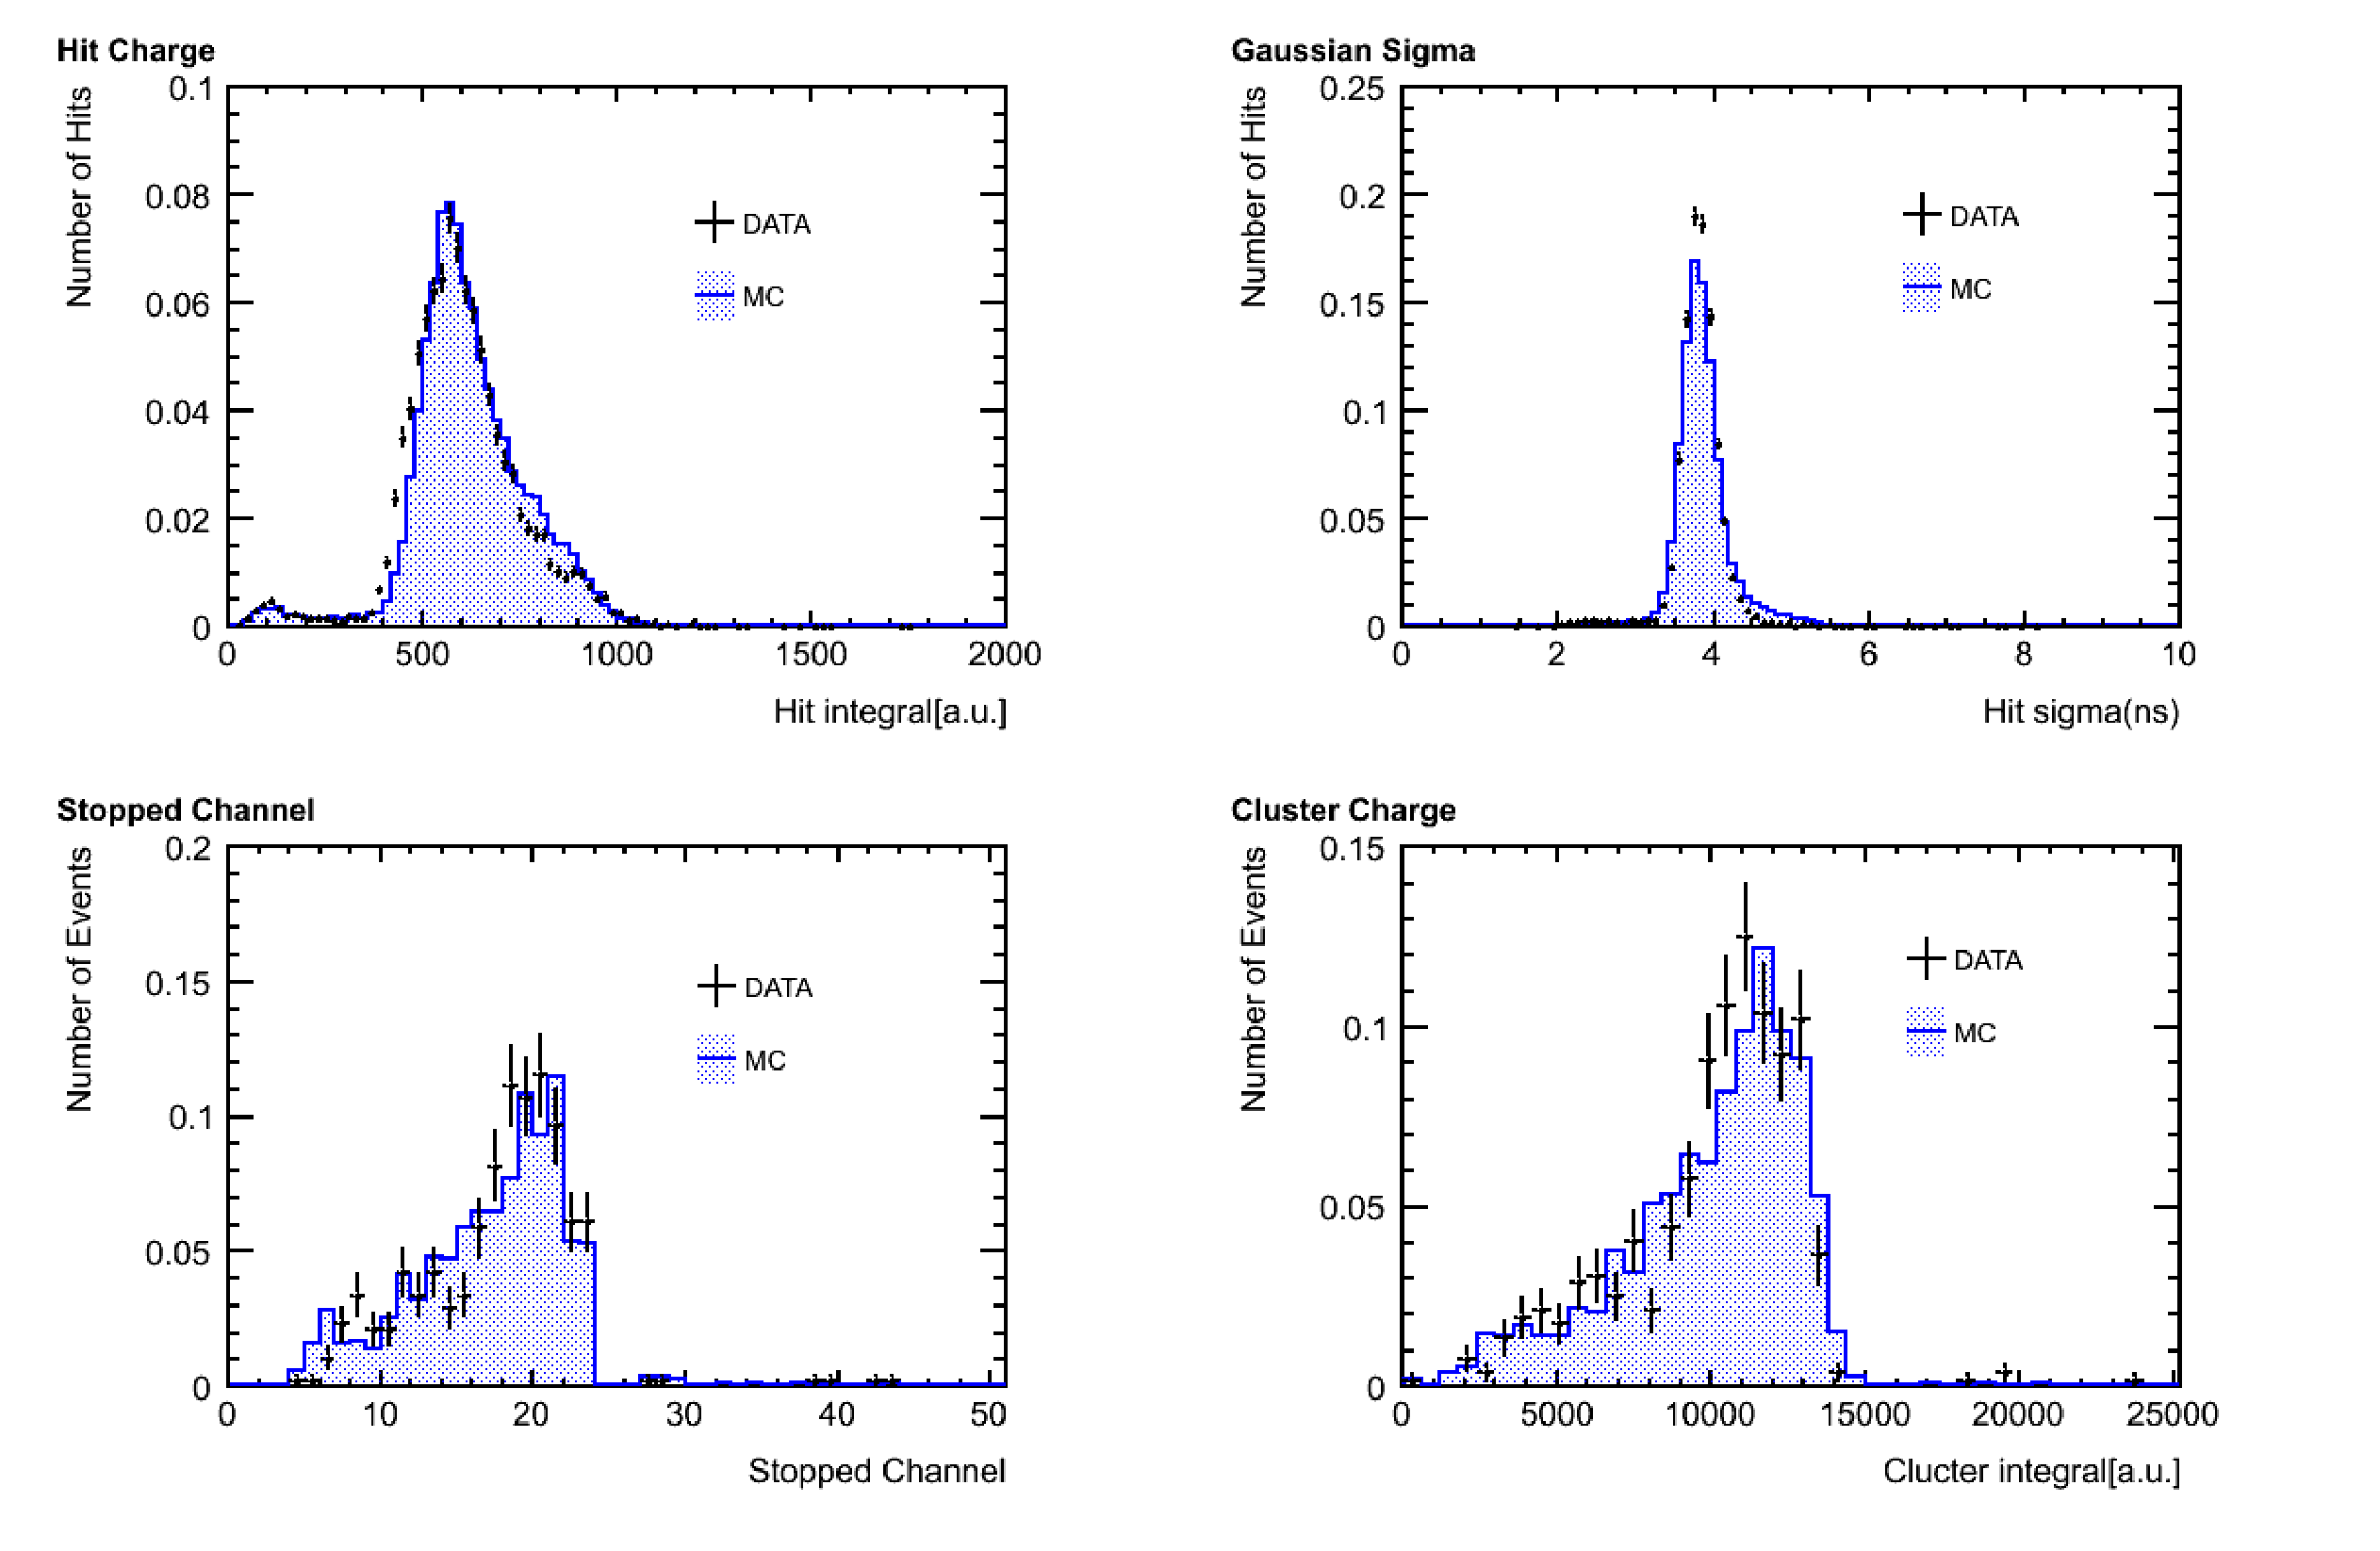
\includegraphics[width=10cm,clip]{./fig/stop_proton_1.eps}
  \caption{DATA-MC comparison of Hit Charge, Hit Sigma, Stopped Channel, Cluster Charge}
  \label{fig:varios_distribution}
\end{figure}

Figure\ref{fig:ADC_distribution} shows the integrated ADC distribution of each channel from stopped channel.
Crosstalk scale is determined by DATA-MC comparison of the left upper histgram,
and this MC distribution agree with DATA well.
The MC distribution of the channels after stopped channel are good agereements with DATA.\\
The left of figure\ref{fig:Mean_comparison} shows the mean of the above distribution of each channel.
The right of figure\ref{fig:Mean_comparison} shows the ratios of DATA/MC.
The ratios are surpressed within 92\%$\sim$100\%.
From this result, we succeed in reproducing the charge response of DATA in high and wide dE/dx region.

\begin{figure}[htbp]
  \centering
  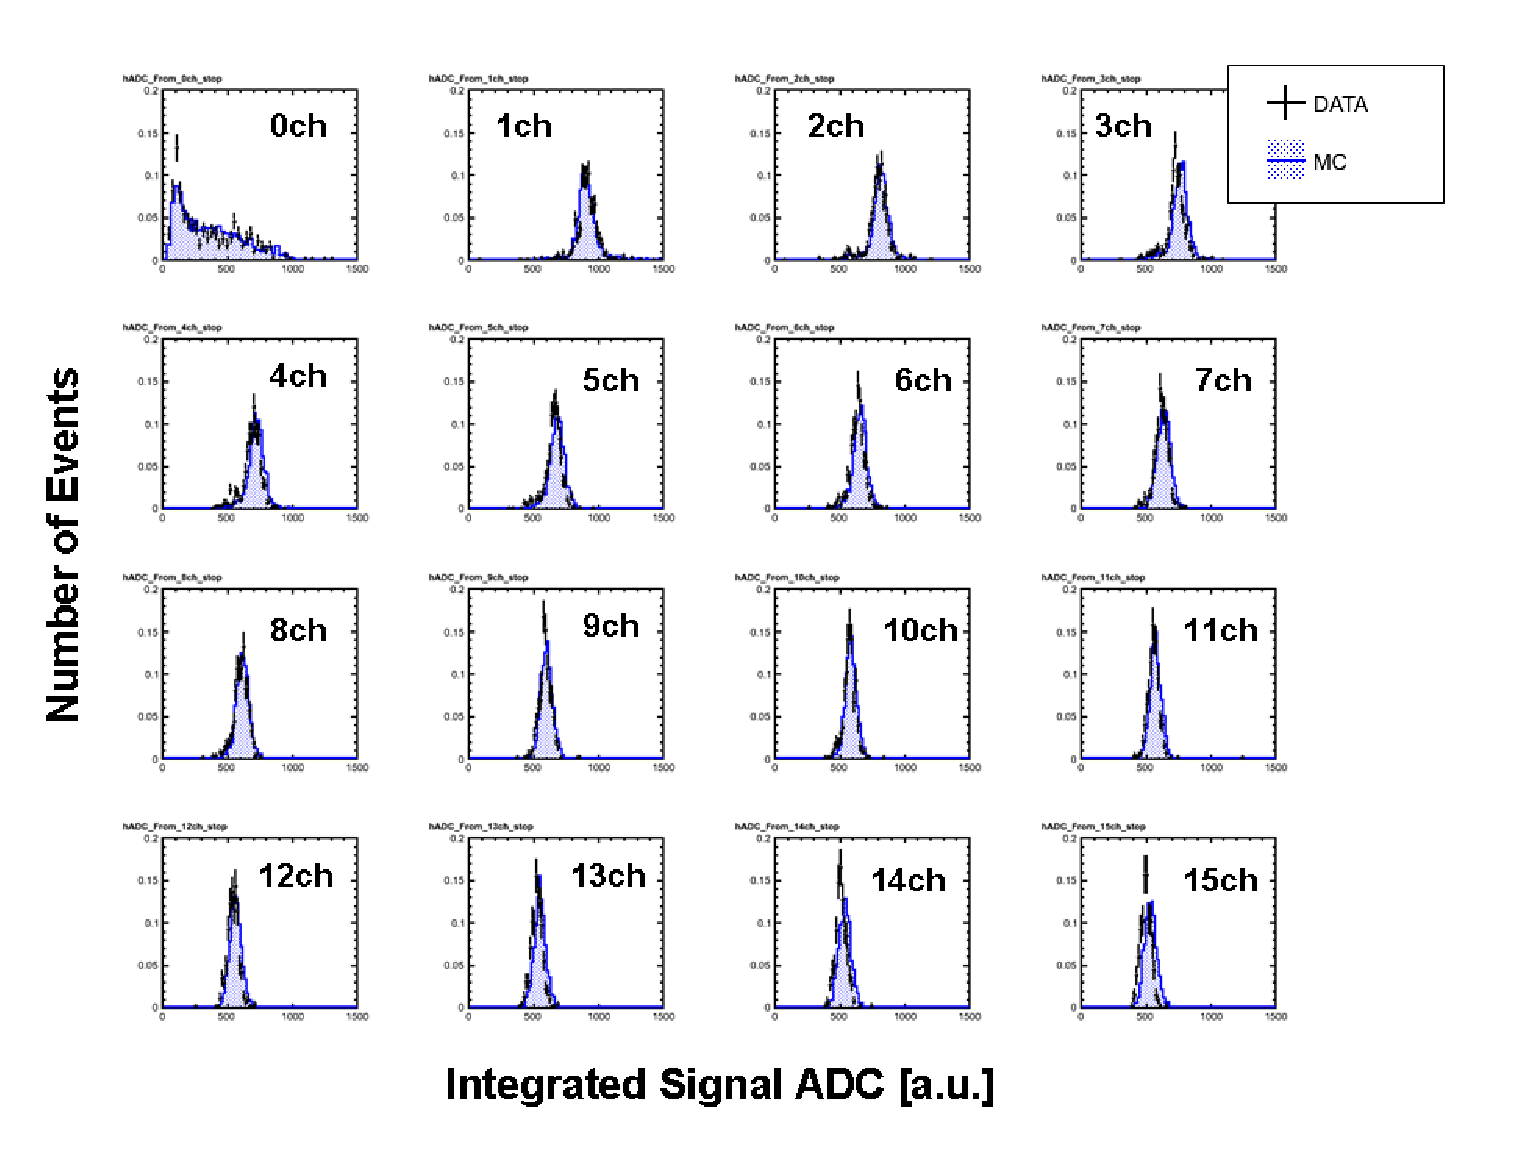
\includegraphics[width=10cm,clip]{fig/stop_proton.eps}
  \caption{Integrared ADC distribution of each channel from stopped channel}
  \label{fig:ADC_distribution}
\end{figure}

\begin{figure}[htbp]
  \centering
  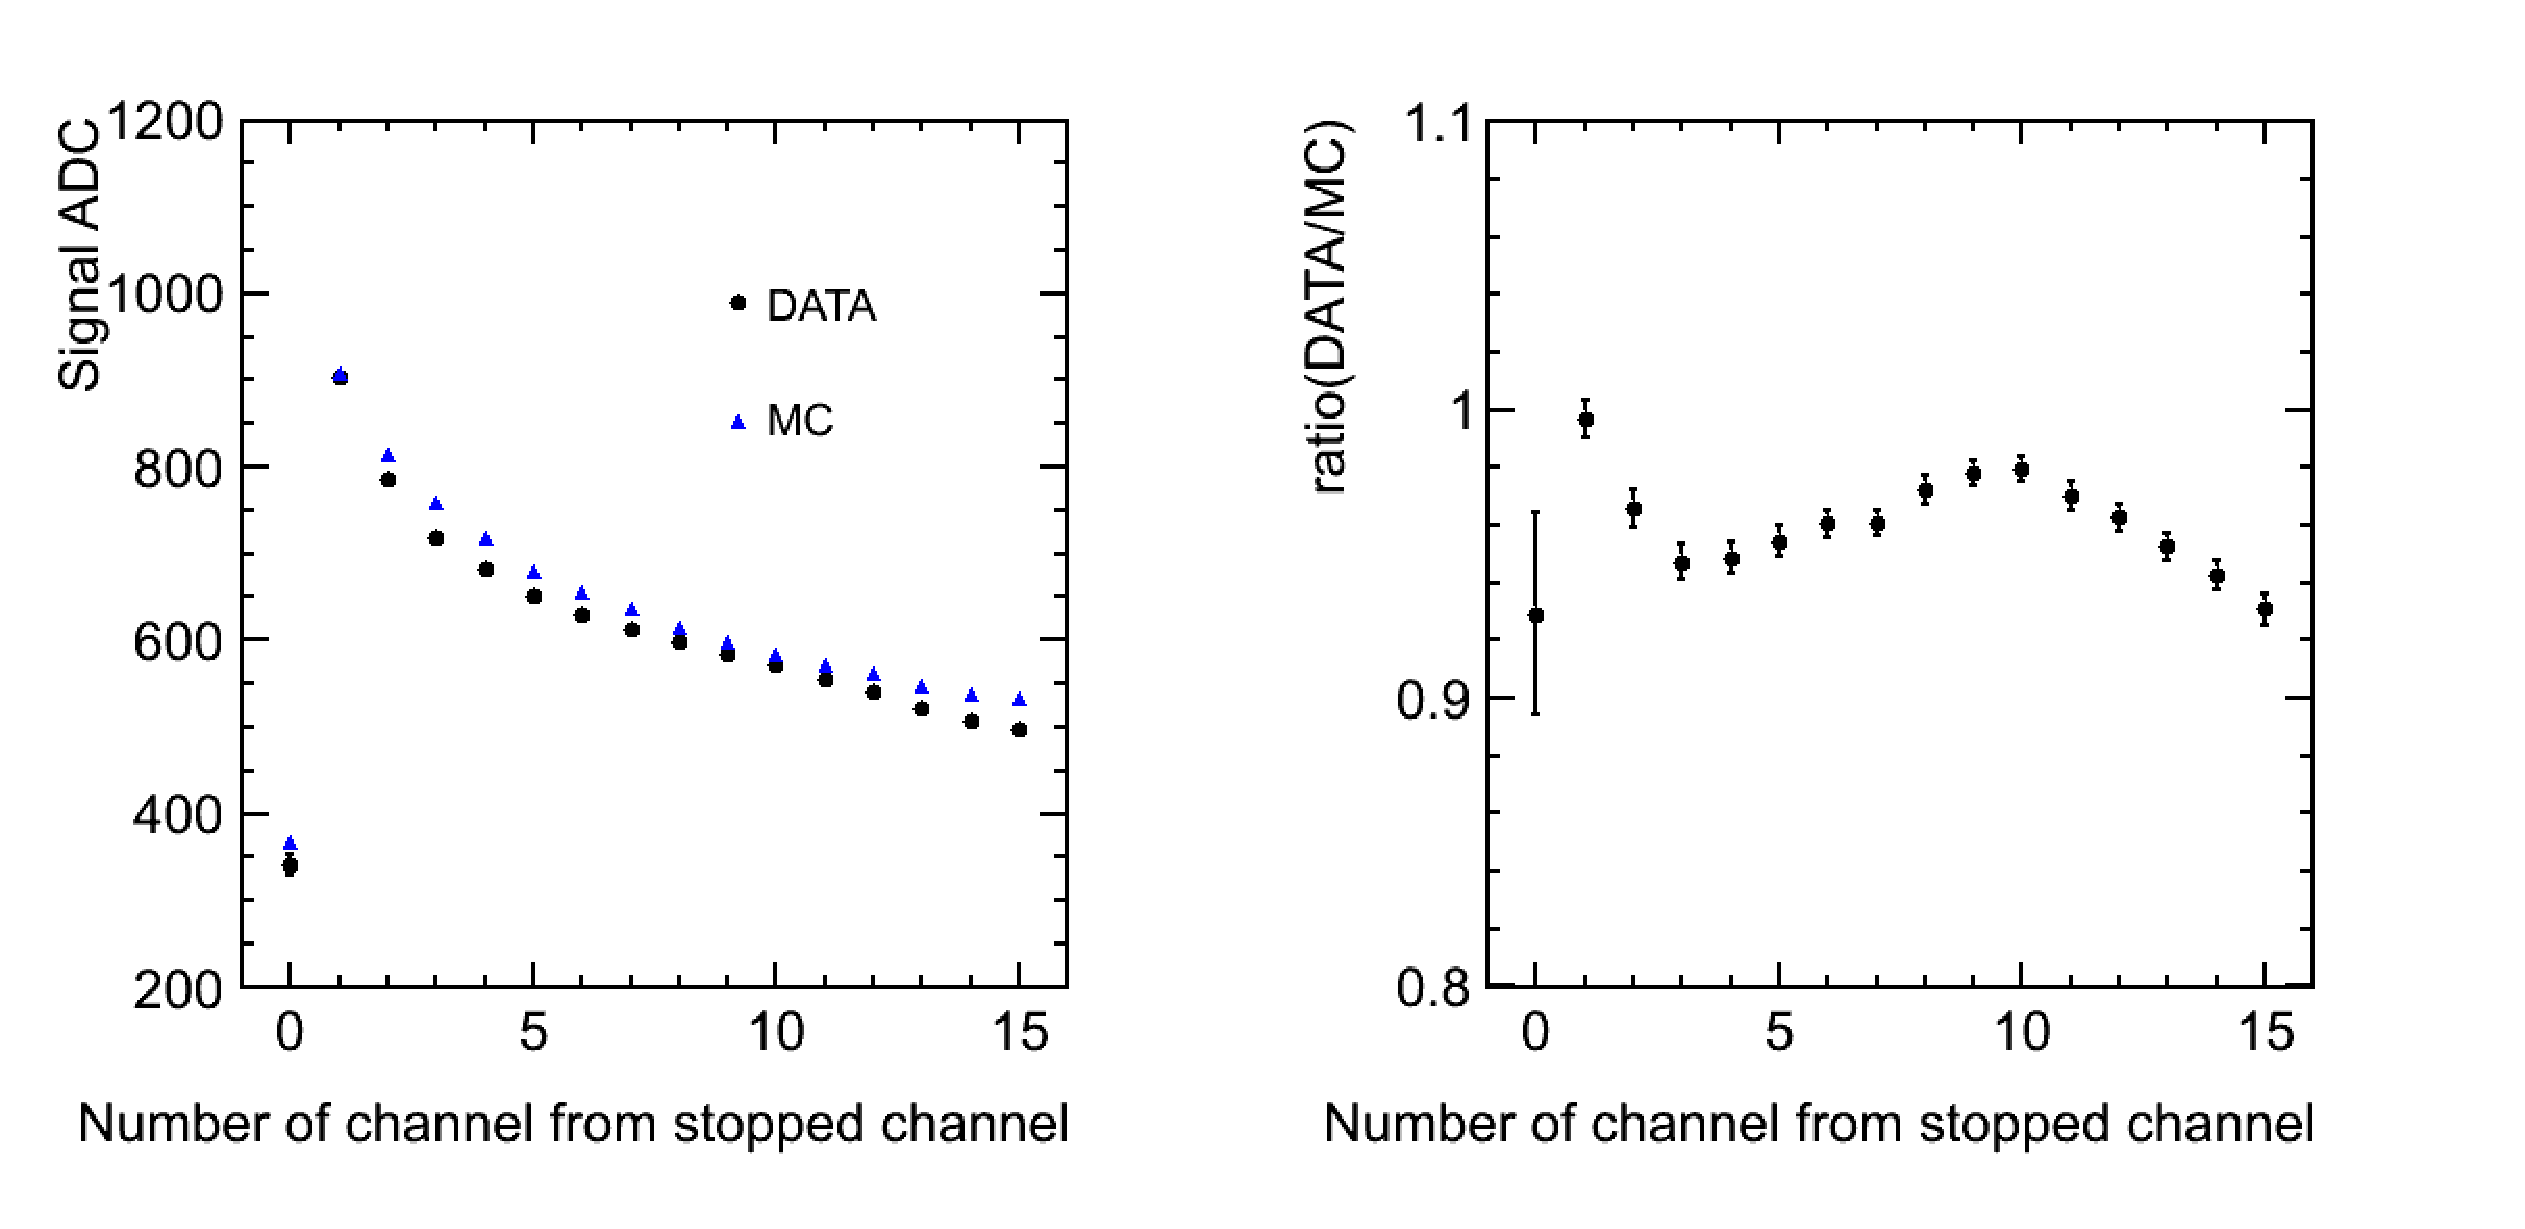
\includegraphics[width=10cm,clip]{fig/stop_proton_3.eps}
  \caption{DATA-MC comparison of the mean of Integrated ADC distribution}
  \label{fig:Mean_comparison}
\end{figure}

\subsection{Stopped Kaon}
